% !TeX spellcheck = en_US
\addscenariosection[subsection]{1}{Rampart coop Campaign $-$ Elixir of Life}{2. Cutthroats}{\images/gelu.png}

\begin{multicols*}{2}

\textbf{Author:} Tm335

\textit{Lord Falorel: Rumor has it that the Ring of Vitality, one of the essential components of the Elixir of Life, is located in the Shantanna region of southern AvLee.
  Time is of the essence, for a Death Knight has been spotted talking to bandits who have long been terrorizing the area, and we believe that he has hired them to find the Ring first.
}


\subsection*{\MakeUppercase{Scenario Length}}

This Scenario plays out over 16 Rounds.

\subsection*{\MakeUppercase{Player Setup}}

\textbf{Player Count:} 2

\textbf{Faction:} Rampart

\textbf{Faction Hero:} Gelu (player 1), and Mephala or Clancy (player 2)

\textbf{Starting Resources:} 15 \svg{gold}, 3 \svg{building_materials}, 1 \svg{valuables}

\textbf{Starting Income:} 10 \svg{gold}, 0 \svg{building_materials}, 0 \svg{valuables}

\textbf{Starting Units:} One player takes 1, the other player takes 2 of the following: a Few Centaurs, a Few Elves, a Few Pegasi

\textbf{Town Buildings:} \bronze\ Dwelling, Citadel

\textbf{Bonus:} One player receives one of the following:
\begin{itemize}
  \item Add Neutral \bronze\ Rogues to your Units.
  \item 6 \svg{gold}
  \item Add the Equestrian Gloves Artifact to your hand.
\end{itemize}

Find the \textbf{Crest of Valor} and \textbf{Angel Wings} Artifacts, and set them aside for later use.

\subsection*{\MakeUppercase{Coop Play Rules}}

In addition to the Cooperative Mode rules (see page 11, ``Cooperative Mode'' in the Core Mission Book), reference the attached \pagelink{Coop Campaign Rules}{Coop Campaign Rules} specific to this campaign.

\subsection*{\MakeUppercase{AI Hero Setup}}

\textbf{Faction:} Necropolis

Before beginning this Scenario, find all Necropolis Neutral Unit Cards in all Neutral Unit Decks, and set them aside.
These will only be used by \textbf{Necropolis Charging Armies}.

Charging Armies move after the Players do, and take the shortest route to the Player that has the Crest of Valor or the Angel Wings.

They ignore everything else, except they will take mines only if flagged by the Rampart player (but they will not backtrack to flag a mine).

\subsection*{\MakeUppercase{Map Setup}}

Take the following Map Tiles and arrange them as shown in the Scenario map layout:

\textbf{2 × Starting (I) Map Tile}
\begin{itemize}
  \item 1 × Rampart (S4)
  \item 1 × Necropolis (S1)
\end{itemize}

\textbf{5 × Far (II--III) Map Tile}
\begin{itemize}
  \item 4 × Castle/Rampart (F10, F12, \#F4 and choose 1 from: F6, F8, \#F8, F11)
\end{itemize}

\textbf{4 × Near (IV--V) Map Tile}
\begin{itemize}
  \item 1 × Castle/Rampart (choose 1 from: N6, N8)
  \item 2 × Dungeon (N2, N5)
\end{itemize}

\subsection*{\MakeUppercase{Heroes Placement}}

Place both Gelu and Mephala/Clancy on the center Field of the Rampart S4 Starting Map Tile.

\subsection*{\MakeUppercase{Victory Conditions}}

Obtain the Ring of Vitality.
Seek out Feredor the Seer (\#F4), who will guide you on how to obtain the Ring of Vitality from the Man in the Southwest (F12).

\subsection*{\MakeUppercase{Defeat Conditions}}

You lose if any of the following occur:
\begin{itemize}
  \item Gelu is defeated in a Combat encounter.
  \item You fail to obtain the Ring of Vitality before the end of Round 16.
\end{itemize}

\subsection*{\MakeUppercase{Timed Events}}

\textbf{\nth{1} Round:}
\begin{itemize}
  \item Read ``Local Warlords'' section.
\end{itemize}

\textbf{\nth{2} Round:}
\begin{itemize}
  \item Read ``First Scourt Report'' section.
\end{itemize}

\textbf{\nth{3} Round:}
\begin{itemize}
  \item Read ``Second Scourt Report'' section.
\end{itemize}

\textbf{\nth{4} Round:}
\begin{itemize}
  \item Read ``The Seer'' section.
\end{itemize}

\textbf{If entering the Witch Hut on \#F4:}
\begin{itemize}
  \item Read ``Feredor the Seer -- first encounter'' section.
\end{itemize}

\textbf{\mbox{\nth{5} and all the following Resource Rounds:}}
\begin{itemize}
  \item Read ``Bandits'' section.
\end{itemize}

\textbf{If you obtain the Crest of Valor or enter N2 or N5 Tile:}
\begin{itemize}
  \item Place Necropolis Heroes on Necropolis Town (S1) and Necropolis Settlement (F1).
\end{itemize}

\columnbreak
\textbf{\nth{7} Round:}
\begin{itemize}
  \item Read ``Terrible Dreams'' section.
\end{itemize}

\textbf{If entering the Witch Hut on \#F4 for the second time:}
\begin{itemize}
  \item Read ``Feredor the Seer -- second encounter'' section.
\end{itemize}

\textbf{If entering the Witch Hut on F12:}
\begin{itemize}
  \item Read ``The Man in the Southwest'' section.
\end{itemize}

\textbf{When you complete the Scenario:}
\begin{itemize}
  \item Read: ``Congratulations! You have passed the Trial! Victory is yours!''
\end{itemize}

\subsection*{\MakeUppercase{Additional Rules}}

During this Scenario:

\begin{itemize}
  \item Gelu cannot surrender.
    Player 2 can surrender.
    If player 2 is defeated in Combat, lose 5 \svg{gold} and both Heroes gain a \svg{morale_negative} token.
    Player 2 Hero is then placed in any Town or Settlement you control, or on a Field adjacent to Gelu.
  \item You cannot recruit a Secondary Hero.
  \item Gain 2 \svg{gold} every time you defeat an Enemy Army.
  \item Players can trade the Crest of Valor and Angel Wings from their hand if they are on adjacent Fields on the map.
\end{itemize}

\subsection*{\MakeUppercase{Combat with Necropolis Charging Armies}}

Every time a Combat encounter starts, draw a Neutral army from the Necropolis Units set aside, with a difficulty level equal to your Hero Level.  % no-check-caps

Every time a Necropolis Charging Army is defeated, they re-appear on the Necropolis Town (S1).
If the Town is occupied, they re-appear on the Necropolis Settlement (F1).
They can move again in the next Resource Round.

\end{multicols*}

\begin{minipage}{\textwidth}
  \vspace{-1em}
  \begin{tikzpicture}[remember picture]
    \node(map)[anchor=center] at (9, -5.5) {
      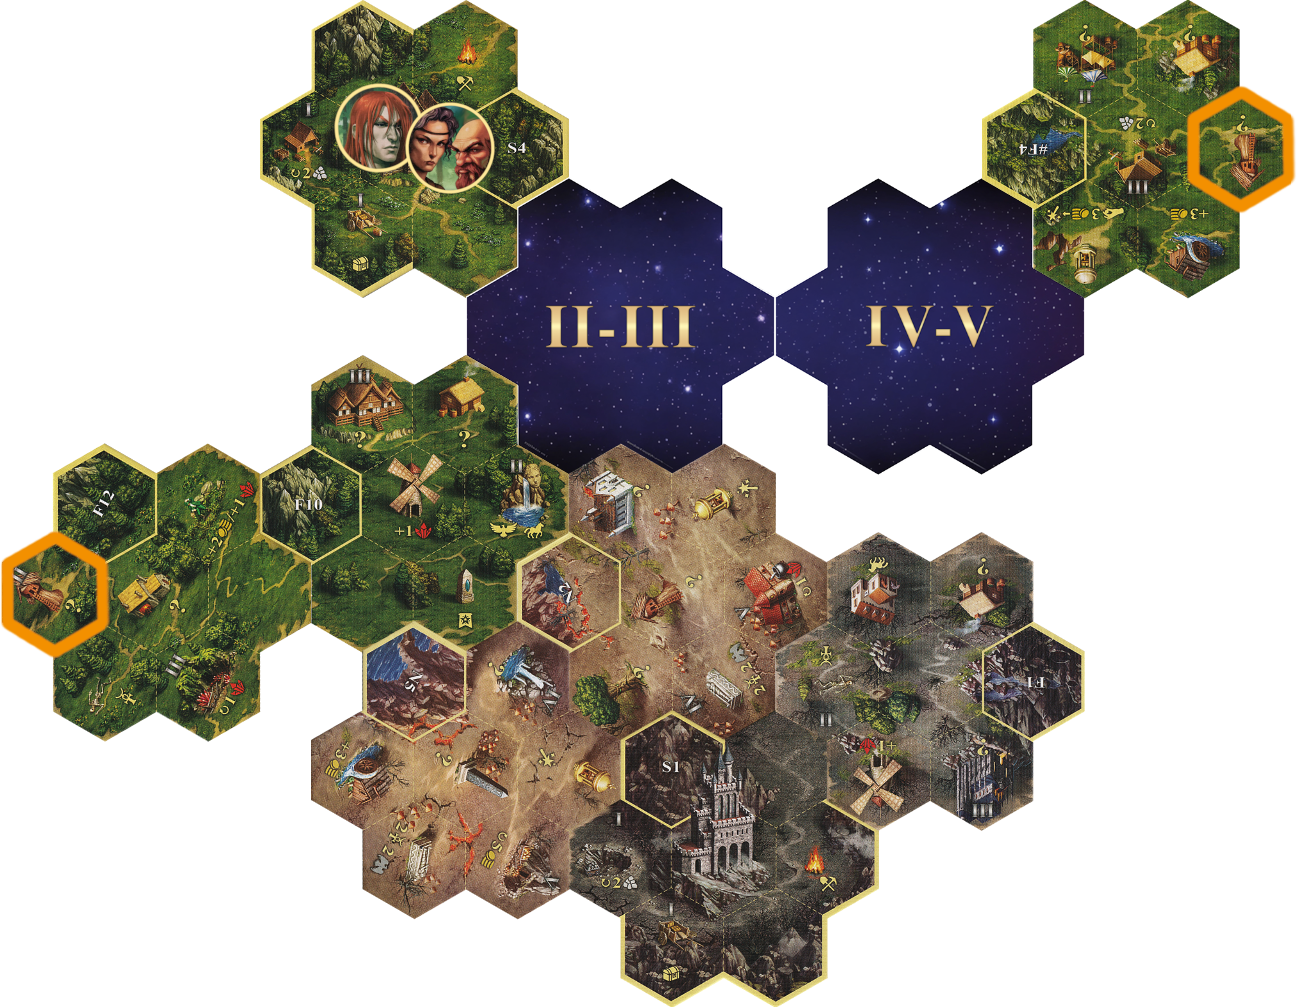
\includegraphics[width=\textwidth]{\maps/rampart_cutthroats.png}
    };
    \node at (3.9,0.6) {\large{{\textbf{\textcolor{darkcandyapplered}{S4}}}}};
    \node at (11.9, -11.6) {\large{{\textbf{\textcolor{darkcandyapplered}{S1}}}}};
    \node at (14.9, -6.6) {\large{{\textbf{\textcolor{darkcandyapplered}{F1}}}}};
    \node at (13.5, 0.6) {\large{{\textbf{\textcolor{darkcandyapplered}{\#F4}}}}};
    \node at (3.7,-4.3) {\large{{\textbf{\textcolor{darkcandyapplered}{F10}}}}};
    \node(f12) at (0.1, -5.5) {\large{{\textbf{\textcolor{darkcandyapplered}{F12}}}}};
    \node at (11.3, -5.5) {\large{{\textbf{\textcolor{darkcandyapplered}{N2}}}}};
    \node at (4.5,-10.5) {\large{{\textbf{\textcolor{darkcandyapplered}{N5}}}}};

    \node(southwest) at (1.2, -9.3) {\large{{\textbf{\textcolor{darkcandyapplered}{Man in the}}}}};
    \node at (1.2, -9.8) {\large{{\textbf{\textcolor{darkcandyapplered}{Southwest}}}}};

    \node(feredor) at (16.9, -3.1) {\large{{\textbf{\textcolor{darkcandyapplered}{Feredor}}}}};
    \node at (16.9, -3.6) {\large{{\textbf{\textcolor{darkcandyapplered}{the Seer}}}}};

    \draw[-Triangle, line width=2.5pt, darkcandyapplered] ($(southwest) + (-0.2, 0.2)$) to[out=135, in=270] ($(f12) + (0.2, -2.0)$);
    \draw[-Triangle, line width=2.5pt, darkcandyapplered] ($(feredor) + (0.5, 0.3)$) to[out=70, in=270] ($(feredor) + (0.7, 1.7)$);
  \end{tikzpicture}
\end{minipage}

\begin{multicols*}{2}

\subsection*{\MakeUppercase{The Story}}

\textbf{Local Warlords}

The warlords in this region are cutthroats and madmen.
They have been looting caravans, razing villages, and butchering garrisons with no thought given to the consequences to their homeland.
They will foolishly sell the Ring of Vitality to the Necromancers and betray their countrymen merely to fill their coffers with gold.
These traitors should be given no quarter and shown no mercy.

\textbf{First Scout Report}

Your spies tell of Feredor, a seer in the Northeast (\#F4) who knows the location of the Ring of Vitality.
Seek him out, learn the Ring's location, and then retrieve it.
Be wary!
The necromancers are also looking for the Ring.

\textbf{Second Scout Report}

Our scouts report that one of the warlords has made contact with the Necromancers and is planning a meeting very soon.
Time is of the essence.
Should that Ring fall into the Necromancers' hands you will need to take it from them by force.
Use whatever means are necessary to keep that Ring safe.
Remember that the best defense is a strong offense: clear this region and defend against any enemy incursion into the Rampart grasslands.

\textbf{The Seer}

The seer in the Northeast is an old wise man named Feredor.
Seek his advice, but be warned he shall not give you the Ring outright.
He is said to issue a test to those who seek the Ring.
Perform whatever task he asks, for you must obtain that Ring.

\textbf{Feredor the Seer -- first encounter}

  Feredor the seer sees the Rampart hero approach and knows he must help them against the hordes of undead.  % no-check-caps
``I can tell you where the Ring can be found.
But you must prove your worthiness.
Bring back the Crest of Valor to me. Now hurry!''

\textcolor{darkcandyapplered}{Roll an Attack Die to determine the \textbf{Crest of Valor}'s location:}
\begin{itemize}
  \item[\textbf{+1}] -- The Crest is on the empty Field of F12
  \item[\textbf{0}] -- The Crest is on the empty Field of F10
  \item[\textbf{-1}] -- The Crest is on the Magic Springs Field of N5.
\end{itemize}

\textbf{Terrible Dreams}

Last night your sleep was wracked with terrible dreams, visions of the dark events to come.
You were haunted by images of a cloaked figure sweeping his skeletal hand across a grassy plain, leaving behind a desolate land overrun by legions of undead monsters.
Sinister laughter echoed throughout your mind and soul.
You awoke, fearful and shaken but still resolved to obtain the Ring of Vitality.

\textbf{Feredor the Seer -- second encounter}

If you are in possession of the Crest of Valor, read: ``There is a man in the southwest (F12) who has it.
He lives in a small hut.
He will only give it to one who he deems worthy.
Bring him these Angel Wings and he will know I sent you.
Move with haste, there is little time.''

\textcolor{darkcandyapplered}{Remove the \textbf{Crest of Valor} from the game, and put \textbf{Angel Wings} into your hand.}

\textbf{The Man in the Southwest}

If you do not have the Angel Wings (in your hand or Deck) and enter this Field, the Man in the Southwest says: ``You are a fool! You are not worthy! Be gone!''

If you are in possession of the Angel Wings (in your hand or Deck) and enter this Field, the Man in the Southwest says: ``Ahhhhh, I see Feredor sent you.
You are worthy.
Here, I give you the Ring of Vitality!''

\textbf{Bandits}

If you haven't secured all mines in all the Grass Map Tiles, bandits have attacked your supply lines and taken valuable resources.

\textcolor{darkcandyapplered}{Lose: 5 \svg{gold}, 1 \svg{building_materials}, 1 \svg{valuables}.}

\vspace*{\fill}

\includegraphics[width=\linewidth, keepaspectratio]{\art/dwarf.jpg}

\end{multicols*}
